\section{Introduction}

\begin{figure}[H]
    \centering
    \begin{subfigure}[b]{0.35\textwidth}
			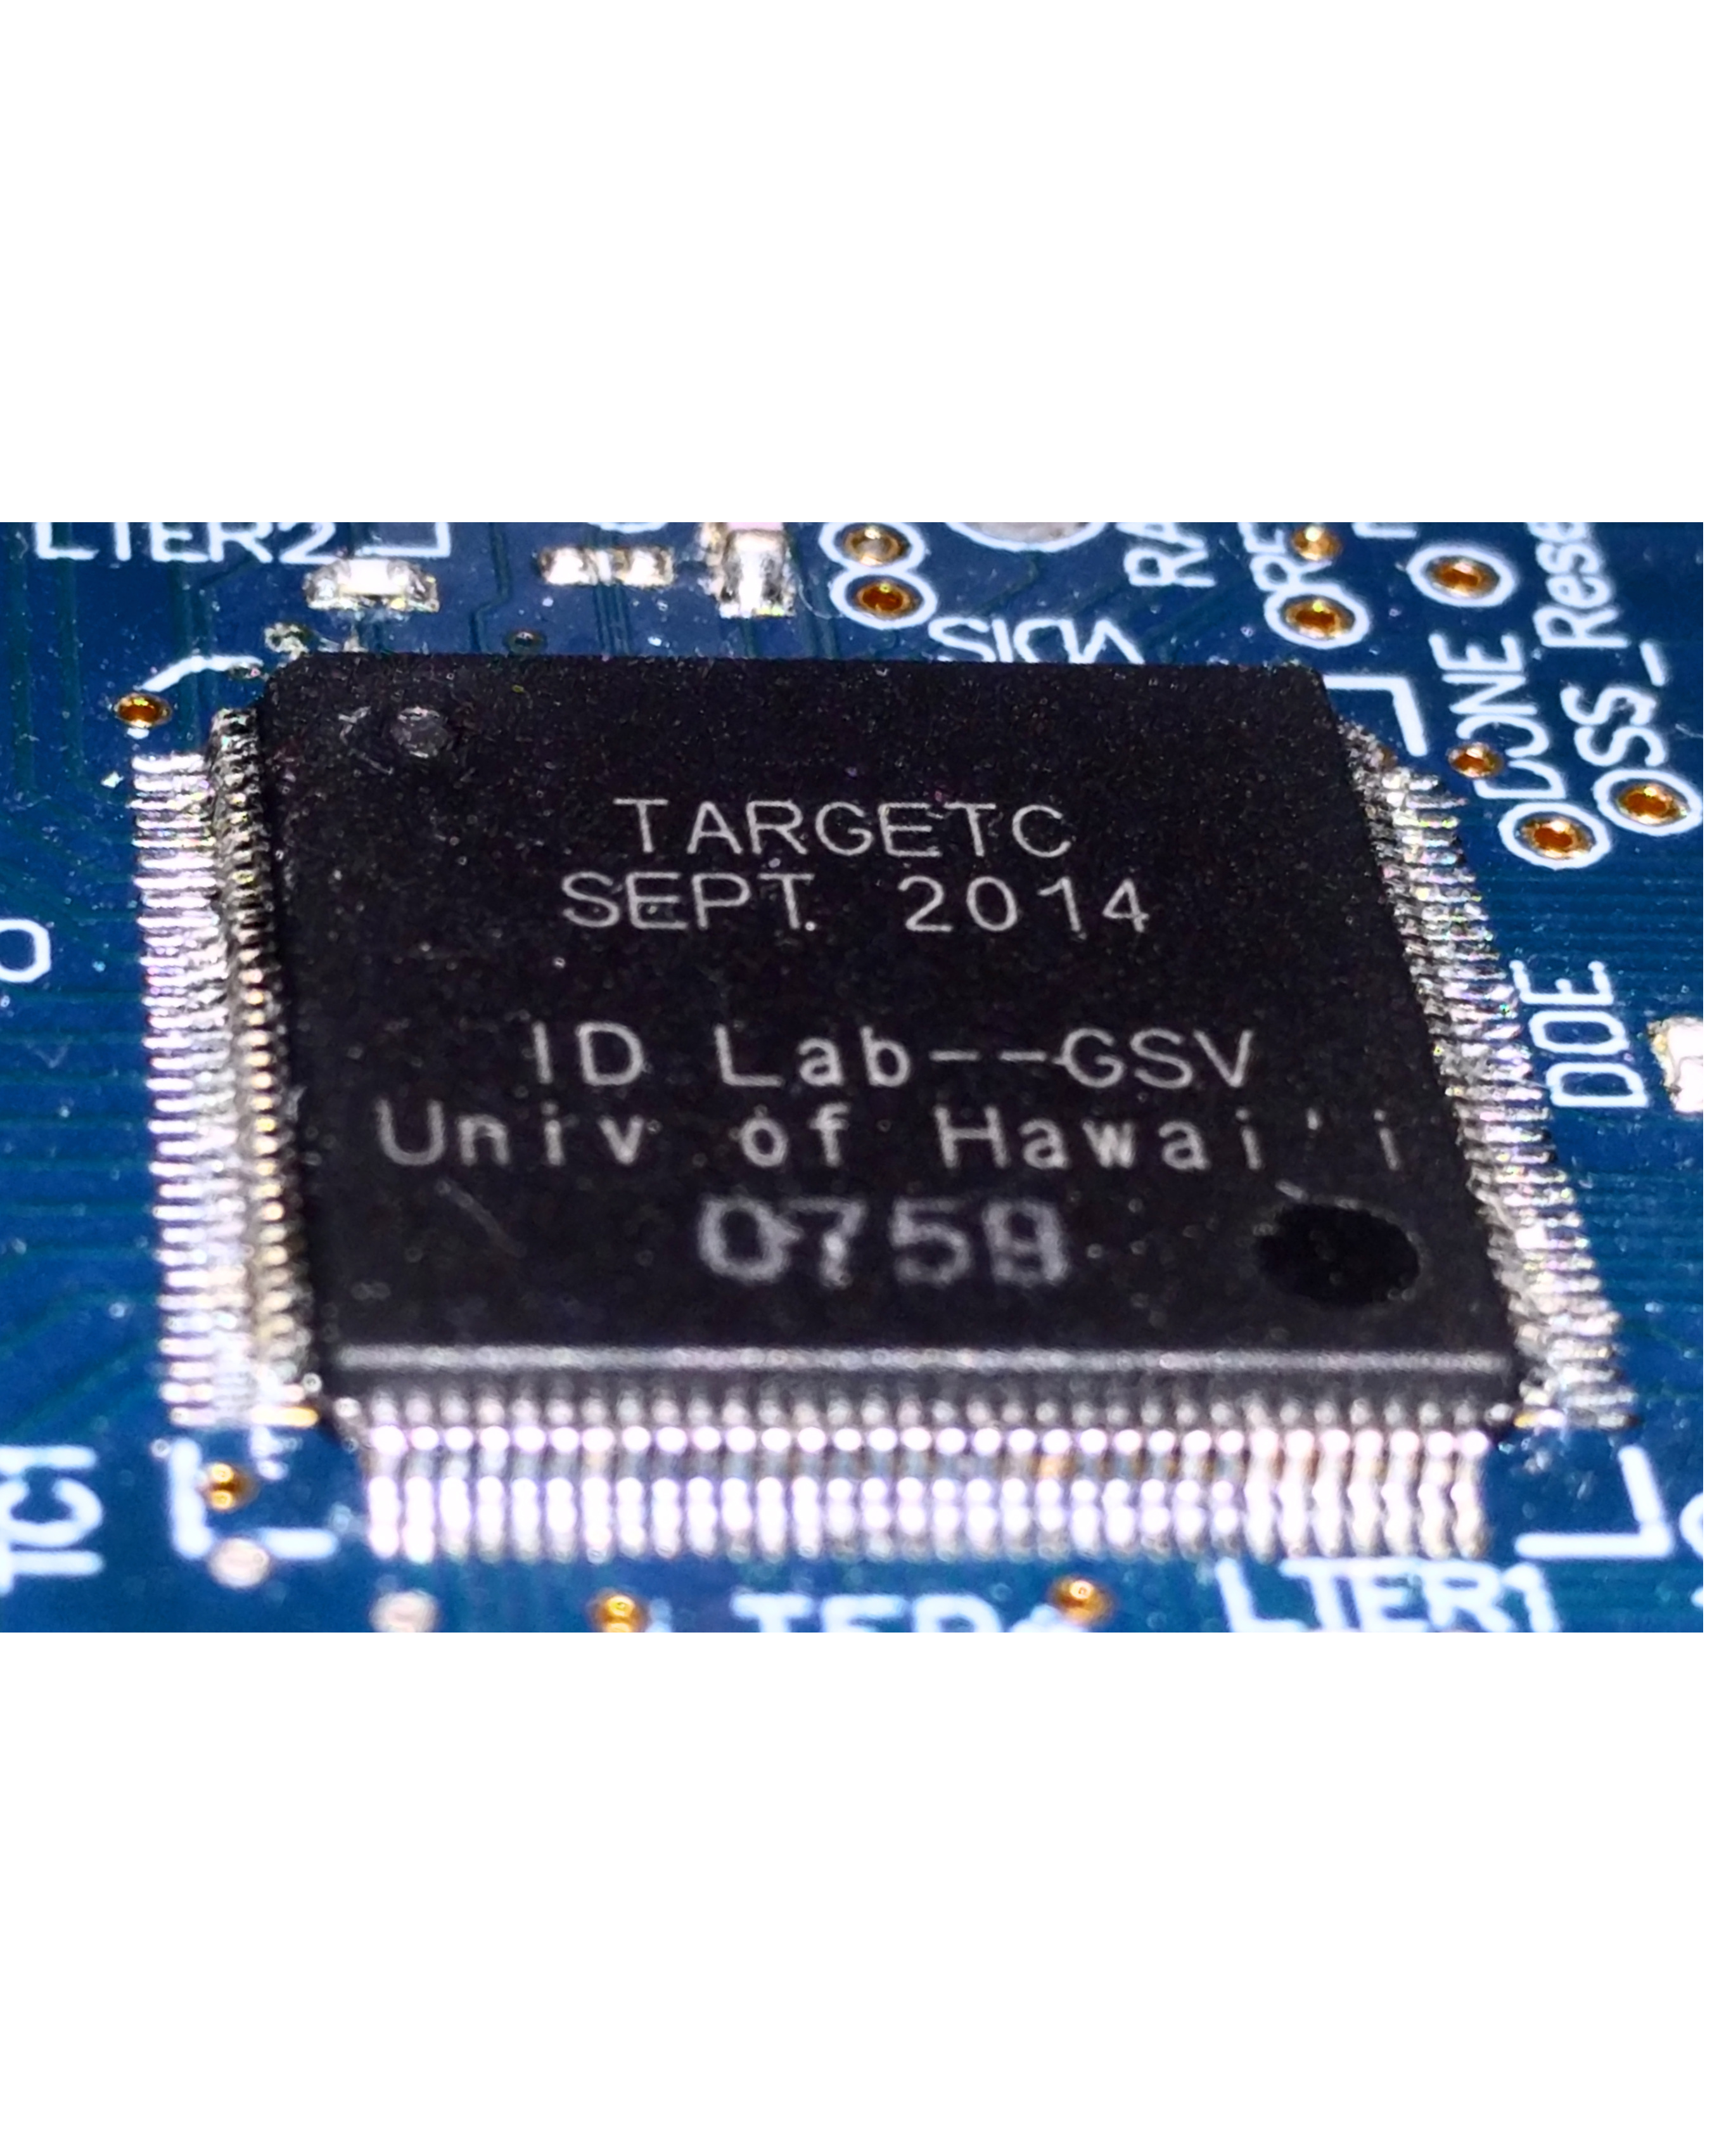
\includegraphics[width=1\textwidth]{figures/targetchip2.jpg}\\
			\caption{\label{fig:TC_chip} Prototype board}
    \end{subfigure}\hfill
    \begin{subfigure}[b]{0.55\textwidth}
			\includegraphics[width=1\textwidth]{figures/TargetC_Top.png}\\
			\caption{\label{fig:TC_top} Top level Schematic}
    \end{subfigure}
    \caption{TARGETC}\label{fig:tctopchip}
\end{figure}

\noindent
TARGET C is a new application-specific integrated circuit (ASIC) of the TARGET family, which stands for TeV Array Readout Gigasample-per-second Electronics without Trigger (TARGET). This circuit is designed by Dr. Gary Varner at the University of Manoa Hawai'i. This ASIC is designed for the readout of signals from photosensors in the cameras of imaging atmospheric Cherenkov telescopes (IACTs) for ground-based gamma-ray astronomy. The TARGET family is composed of :
\begin{itemize}
  \item TARGET 5
  \item TARGET 7
  \item TARGET X
  \item TARGET C
\end{itemize}

\noindent
The main difference from the TARGETX to C is the control over storage cells and the triggering system, these details are explained later in this document.

\newpage
\section{Overall Architecture}
The TARGETC can sample 2 x 32 samples x 16 channels at once. To do so a capacitor array composed of 64 sampling capacitors (SaC0 to SaC63) which are charged by a switch command signal generated by the SSTIN provided by the FPGA and SSPIN clock internally generated,  see figure \ref{fig:capacitorarray2}. For simplicity, this illustration only shows the channel RFIN\_1 but there is 16 of them in parallel, consequently all sampling on the 16 channels is done at the same time. The sampling frequency depends on the SSTIN signal, generally the clock period is set to 64 ns. Each switch command is delayed by 1ns, but the width of the pulse is larger than 1ns giving the time for the capacitor to charge up. The delay circuit is composed of two inverters, one fixed delay and the other is adjustable (coarse and fine tune). Adjustment value is determined by a DLL (Delay Lock Loop) or can be written in a register. The signal SW0 is formed by logic combination of the superposition of two clocks and is enabled 1ns earlier than SW1 signal and 2ns earlier than SW2  signal, see figure \ref{fig:pulse1ns}. Assuming that each capacitor is switched ON and OFF at 1ns of interval, the input signal is sampled at a frequency of 1 Giga-Sample per second (1GS/s).

\begin{figure}[H]
\centering
\includegraphics[width=1\textwidth]{figures/capacitor_array.png}\\
\caption{\label{fig:capacitorarray2} Capacitor array for sampling analog input}
\end{figure}

\begin{figure}[H]
\centering
\includegraphics[width=1\textwidth]{figures/wavedrom/switchPulse.png}\\
\caption{\label{fig:pulse1ns} Switch command Pulse Generator for 1ns delay between samples}
\end{figure}

\noindent
The storage address is commanded by the FPGA side using the ASIC input pins, WR\_COL\_SEL(5:0) and WR\_ROW\_SEL(1:0). The storage location is formed of capacitors (StC0 to StC63). The location addressed is latched onto the internal address bus by a write address sync (internal signal). Once the address is stable inside the ASIC, a second internal signal is enabled (write strobe). This signal switches ON and OFF the transmission lines to store the analog value from SaC0-SaC63 into the storage cells StC0-StC63. The 64 samples are stored in two different parts of the analog memory. The ASIC separates the 64 samples into 2 windows of 32 samples (EVEN and ODD part). The LSB bit for row selection is this EVEN and ODD window select. The total analog memory is 32 samples x 8 rows x 64 columns = 16K samples. The FPGA must keep track which part of memory is occupied and which is free. This write command is done in parallel for the 16 channels of the TARGETC.

\begin{figure}[H]
\centering
\includegraphics[width=1\textwidth]{figures/storagearea2.png}\\
\caption{\label{fig:storagearea} Analog storage area of 16K cells per channel}
\end{figure}

\noindent
The digitalization is performed in parallel for the 32 samples per channel. It is triggered by sending the address through a serial communication (RDAD\_clk, RDAD\_sin and RDAD\_dir). The address is decoded and triggers a read command which turns on the Wilkinson comparators of the memory location (normally off for power consumption).

\noindent
The Wilkinson ramp is started by enabling the ramp signal. The ramp parameters are defined by a simple linear function $y = a*x+b$. The argument $a$ is the slope of the ramp commanded by the ISEL register. The second argument $b$ is defining the offset voltage of the function, this offset is the voltage discharge of the wilkinson capacity defined by a register VDISH. The Wilkinson ADC compares the voltage of a capacitor to a digital counter, when the comparison is equal the analog value is represented by the digital value inside the counter. Therefore the frequency at which this counter is increment must be linked to charge speed of the capacitor. So the Wilkinson clock period multiplied by the counter's length defines the total time of charge. The gray code is used for changing only 1 bit at the time and avoiding dangerous transition levels and meta-stabilities, like for example the transition from 127 to 128 ($01111111_{2}$ to $10000000_{2}$).\\The figure \ref{fig:vramp} shows the different actors for varying the charge parameters of the capacitor.

\begin{figure}[H]
\centering
\includegraphics[width=0.8\textwidth]{figures/vramp.png}\\
\caption{\label{fig:vramp} Principle scheme for Vramp}
\end{figure}

\noindent
Once the voltage of the charge capacitor is above the storage cell voltage, the comparator switches from LOW to HIGH. This transaction latches the content of the Gray counter into a sample register. This digital value is the representation of the analog value in memory. The digitization process is finished. The eDONE signal is pulled high when all conversions are over. To put in another way, all comparators have switched from LOW to HIGH, when the 32 samples of each 16 channels are digitized. Only then is the eDONE signal pulled HIGH, see Figure \ref{fig:edone}. \\

\begin{figure}[H]
\centering
\includegraphics[width=1\textwidth]{figures/edone.png}\\
\caption{\label{fig:edone} Logic circuit for eDONE signal}
\end{figure}

\noindent
All samples of the 16 channels are serialized on the Data output pins DO0 to DO15. The SS\_INCR signal pulled HIGH loads a sample register onto the data line, on the HIGH to LOW transition the data line is latched into the shift register. This generated pulse on SS\_INCR will also increase the sample counter, on the next HIGH transition the next sample will be loaded and so on.

\newpage
\begin{figure}[H]
\centering
\includegraphics[width=1.3\textwidth, angle = 90]{figures/digit2.png}\\
\caption{\label{fig:digit2} Full Readout and Digitalization}
\end{figure}

\newpage
\noindent
The ASIC has a built-in Delay Lock Loop, that once enabled and stable, will adjust the timing to temperature fluctuation. The figure \ref{fig:dll} illustrates the DLL's different parameters.

\begin{figure}[H]
\centering
\includegraphics[width=0.9\textwidth]{figures/dll.png}\\
\caption{\label{fig:dll} Principle scheme for DLL}
\end{figure}

\newpage
\section{New Features}
\subsection{External Trigger}
The first difference from previous design like TARGETX, which is used in Belle II detector (over 20k channels), is the triggering system. On the TARGET X, the trigger circuit is internally managed and has the capabilities to trigger on any of the 16 channels. In TARGETC design the trigger system is removed, which means that the full control comes back to the FPGA or the interfacing device. As a consequence, the WATCHMAN TARGETC prototype board uses four operational amplifiers used as comparators. Four independent and adjustable threshold voltages are compared the highest gain lines (x10), which are Channel input 3, 7, 11 and 15 (see figure \ref{fig:TC_trigger}).

\begin{figure}[H]
\centering
\includegraphics[width=0.5\textwidth]{figures/ProtoTriggerSmall.png}\\
\caption{\label{fig:TC_trigger} Principle scheme for External Trigger Circuit on the TARGET C Prototype}
\end{figure}

\subsection{External Storage Control}
The second difference from previous designs is the control over the analog memory storage. Earlier versions used an internal counter with a write enable, the parameter was turned OFF if the cell was not to be re-written. Unfortunately this also means that the data at that exact moment is not written in any memory or anywhere else, it is simply lost. In order to avoid this issue, the control circuit is brought out of the TARGET and left to the user to implement any algorithm to deal with storage control.
